\chapter{计数原理与排列组合}
\label{chap:counting-principles}

\begin{learninggoals}
  \begin{enumerate}
    \item 能判断一项任务应分类还是分步，并在分类互斥、步骤完整的前提下计数；
    \item 掌握排列数、组合数及其恒等式，能解释公式中的每一个因子与除数；
    \item 会用捆绑、插空、选位、排除和容斥处理位置限制；
    \item 能区分对象与容器是否相同、是否允许为空，据此选择分组、满射或隔板模型；
    \item 能把错排、格路、组合几何与环形染色还原为可核对的基本计数过程。
  \end{enumerate}
\end{learninggoals}

\section{分类与分步}

\begin{lawbox}[分类加法与分步乘法]
  完成一件事若有互不重叠的 $r$ 类办法，第 $i$ 类有 $m_i$ 种，则办法总数为
  \[
    m_1+m_2+\cdots+m_r.
  \]
  若完成一件事必须依次经过 $r$ 个步骤，第 $i$ 步有 $m_i$ 种选择，且每组步骤选择都唯一确定一种完成方式，则办法总数为
  \[
    m_1m_2\cdots m_r.
  \]
  分类要求“每一种结果恰落入一类”，分步要求“每一步都完成后才得到结果”。
\end{lawbox}

\begin{examplebox}[原稿型：书架取书]
  一个书架的三层分别放有 $3$ 本数学书、$2$ 本语文书和 $2$ 本英语书，书均不相同。
  \begin{enumerate}
    \item 任取一本书，有多少种取法？
    \item 数学、语文、英语各取一本，有多少种取法？
  \end{enumerate}

  \textbf{解：}第 (1) 问按书的学科分类，每次只进入一类，故有
  \[
    3+2+2=7
  \]
  种。第 (2) 问必须完成三次选择，故有
  \[
    3\times2\times2=12
  \]
  种。两问使用相同数据，但“取一本”是分类，“各取一本”是分步。
\end{examplebox}

\begin{examplebox}[原稿型：四位号码的首位限制]
  用数字 $0,1,\ldots,9$ 编写四位号码，数字允许重复。
  \begin{enumerate}
    \item 若号码允许以 $0$ 开头，共有多少个？
    \item 若把它看成四位正整数，共有多少个？
  \end{enumerate}

  \textbf{解：}号码的四个位置各有 $10$ 种选择，共 $10^4$ 个。四位正整数的首位不能为 $0$，故有
  \[
    9\times10^3=9000
  \]
  个。

  \textbf{辨析：}“四位号码”和“四位数”不是同一个计数对象；是否允许首位为 $0$ 必须由题意决定。
\end{examplebox}

\begin{corollarybox}[交集不能被重复计数]
  若对象可能同时属于两类，仅把两类数目相加会把交集算两次。对有限集合 $A,B$，
  \[
    |A\cup B|=|A|+|B|-|A\cap B|.
  \]
  若要分别从 $A$、$B$ 中选人而同一人不能兼任，还要按“是否选到交集中的人”分类。
\end{corollarybox}

\begin{examplebox}[原稿型：两种技能有交集]
  某组 $9$ 人中，$7$ 人会技能甲，$3$ 人会技能乙，恰有 $1$ 人两种技能都会。现选两名不同的人，一人负责甲、一人负责乙，共有多少种选法？

  \textbf{解：}把人员分成“只会甲”$6$ 人、“两种都会”$1$ 人、“只会乙”$2$ 人。
  \begin{itemize}
    \item 若不选兼会者，只能从前后两类各取一人，有 $6\times2$ 种；
    \item 若选兼会者，他可以负责其中一种技能，另一人从相应的专门人员中选，有 $6+2$ 种。
  \end{itemize}
  因而共有
  \[
    6\times2+6+2=20
  \]
  种。这里的分类同时解决了“交集重复”和“一人不能兼任”两个问题。
\end{examplebox}

\begin{examplebox}[原稿例：2520 的约数]
  求 $2520$ 的正约数个数和偶正约数个数。

  \textbf{解：}
  \[
    2520=2^3\cdot3^2\cdot5\cdot7.
  \]
  任一正约数可唯一写成 $2^\alpha3^\beta5^\gamma7^\delta$，其中
  \[
    0\le\alpha\le3,\quad0\le\beta\le2,
    \quad0\le\gamma,\delta\le1.
  \]
  因而正约数共有
  \[
    4\times3\times2\times2=48
  \]
  个。偶约数要求 $\alpha\ge1$，故共有
  \[
    3\times3\times2\times2=36
  \]
  个。
\end{examplebox}

\begin{examplebox}[原稿例：四区地图相邻异色]
  四个区域首尾相邻成环，使用五种颜色染色，要求有公共边的区域颜色不同。求染色数。

  \begin{center}
  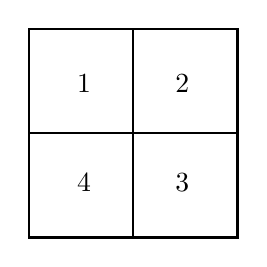
\begin{tikzpicture}[scale=.78]
    \draw[thick] (-1.7,-1.7) rectangle (1.7,1.7);
    \draw[thick] (-1.7,0)--(1.7,0) (0,-1.7)--(0,1.7);
    \node at (-.8,.8) {$1$}; \node at (.8,.8) {$2$};
    \node at (.8,-.8) {$3$}; \node at (-.8,-.8) {$4$};
  \end{tikzpicture}
  \end{center}

  \textbf{解法一：按第 $3$ 区是否与第 $1$ 区同色分类。}先染第 $1,2$ 区，有 $5\times4$ 种。
  若第 $3$ 区与第 $1$ 区同色，第 $4$ 区有 $4$ 种；若不同，第 $3$ 区有 $3$ 种，第 $4$ 区有 $3$ 种。故
  \[
    5\times4\,(4+3\times3)=260.
  \]

  \textbf{解法二：按实际使用的颜色数分类。}使用 $2,3,4$ 种颜色的方案数分别为
  \[
    5\times4,\qquad
    2\times5\times4\times3,\qquad
    5\times4\times3\times2,
  \]
  相加仍得 $260$。

  \textbf{方法启示：}图形染色不是简单地逐块乘“剩余颜色数”。后染区域同时与两个已染区域相邻时，可选颜色数取决于那两个区域是否同色，必须分类。
\end{examplebox}

\begin{examplebox}[原稿例：相邻两天不能由同一人值班]
  五个人安排星期一至星期五的值班，每天一人，同一人不能连续值班两天。求安排数。

  \textbf{解：}星期一有 $5$ 种选择；此后每天只需避开前一天的人，各有 $4$ 种选择。因此共有
  \[
    5\times4^4=1280
  \]
  种。一个人可以隔天再次值班，不能误当作无重复排列。
\end{examplebox}

\begin{examplebox}[原稿型：金额数不等于取法数]
  手中各有有限张 $50$ 元、$20$ 元、$10$ 元和 $1$ 元纸币。问能组成多少种不同金额。

  \textbf{解：}应先把前三种纸币折算成“十元单位”。不同选法可能组成同一金额，例如一张 $20$ 元与两张 $10$ 元，不能直接把各面额的取法数相乘。正确做法是：
  \begin{enumerate}
    \item 先确定可组成的十元整数是否连续，并列出缺口；
    \item 再把可用的一元张数加到每个十元金额上；
    \item 对零元和区间交叠处去重。
  \end{enumerate}
  这道原稿题的作用是提醒：计数对象是“金额”，不是“纸币组合”。
\end{examplebox}

\section{排列与位置限制}

\begin{definitionbox}[排列、排列数与全排列]
  从 $n$ 个不同元素中取出 $m$ 个，按照一定次序排成一列，称为一个 $m$ 元排列。排列数记为
  \[
    A_n^m=n(n-1)\cdots(n-m+1)=\frac{n!}{(n-m)!}.
  \]
  当 $m=n$ 时称为全排列，$A_n^n=n!$，并约定 $0!=1$。
\end{definitionbox}

\begin{examplebox}[原稿例：十点取两点]
  平面上有 $10$ 个点，其中任意三点不共线。
  \begin{enumerate}
    \item 过其中两点作直线，可作多少条？
    \item 以其中两点为起点、终点作有向线段，可作多少条？
  \end{enumerate}

  \textbf{解：}直线不区分两点次序，有 $\binom{10}{2}=45$ 条；有向线段区分起点和终点，有
  \[
    A_{10}^2=10\times9=90
  \]
  条。是否区分次序，正是组合与排列的分界。
\end{examplebox}

\begin{corollarybox}[四类位置限制]
  \begin{itemize}
    \item \textbf{相邻：}把必须相邻的对象捆成一个整体，整体内部还要排列；
    \item \textbf{不相邻：}先排其余对象，再把受限对象插入形成的空位；
    \item \textbf{不全满足：}常用总数减去违例数；
    \item \textbf{多个限制交叠：}用分类或容斥，不要把两个“坏事件”简单相加。
  \end{itemize}
  捆绑和插空的关键不是记公式，而是画出最后可用的“整体”或“空位”。
\end{corollarybox}

\begin{examplebox}[原稿方法：三男四女排队]
  三名男生、四名女生排成一列，七人互不相同。
  \begin{enumerate}
    \item 三名男生必须相邻；
    \item 三名男生互不相邻；
    \item 男女相间；
    \item 三名男生不全相邻。
  \end{enumerate}

  \textbf{解：}
  \begin{enumerate}
    \item 把三名男生看作一个整体，与四名女生共五个对象，故有 $5!\,3!$ 种。
    \item 先排四名女生形成五个空位，再选三个空位放男生，故有 $4!A_5^3$ 种。
    \item 因女生多一人，只能是女男女男女男女，故有 $4!3!$ 种。
    \item 从全部排列中减去男生全相邻的排列，得 $7!-5!3!$ 种。
  \end{enumerate}
\end{examplebox}

\begin{examplebox}[原稿型：两个相邻条件的容斥]
  七人排队，要求甲、乙不相邻，丙、丁也不相邻。求排法数。

  \textbf{解：}设 $E_1$ 为甲乙相邻，$E_2$ 为丙丁相邻。则
  \[
    |E_1|=|E_2|=2\cdot6!,
    \qquad |E_1\cap E_2|=2^2\cdot5!.
  \]
  所求为
  \[
    7!-2(2\cdot6!)+2^2\cdot5!.
  \]
  最后一项必须加回，因为两对都相邻的排列在前一步被减了两次。
\end{examplebox}

\begin{examplebox}[原稿例：七盆花中的两盆菊花]
  七盆不同的花排成一列，其中两盆是菊花。要求两盆菊花不相邻且都不在两端，求排法数。

  \textbf{解法一：选位。}可供菊花使用的是中间五个位置。从中选两个不相邻位置，共
  \[
    \binom52-4=6
  \]
  组；两盆菊花互换，其他五盆排列，故有 $6\cdot2!\cdot5!$ 种。

  \textbf{解法二：先排其他花再插空。}先排五盆非菊花。去掉两端空位后，中间有四个空位；选两个不同空位并安排两盆菊花，有
  \[
    5!A_4^2
  \]
  种，与上式相等。

  \textbf{解法三：排除。}先计两盆菊花不相邻的全部排法 $5!A_6^2$，再减去至少一盆位于端点的情形；分类时需把“两盆恰在两端”加回。此法可行，但交叠项更多。

  \textbf{方法启示：}同一道题中，选位法直接描述合法位置，插空法直接构造合法排列；排除法适合坏情形比好情形更容易数时使用。
\end{examplebox}

\begin{examplebox}[原稿型：主客场、信号与赠书]
  \begin{enumerate}
    \item $14$ 支球队两两进行主客场比赛，比赛总场数是多少？
    \item $8$ 个不同信号位中安排 $4$ 个不同信号，有多少种安排？
    \item 从 $5$ 本不同的书中取 $3$ 本，依次送给三个不同的人，每人一本，有多少种送法？若书的种类可以重复选择，又是多少？
    \item 红、黄、蓝三面不同的旗帜，从中取一面、两面或三面竖直悬挂表示信号，共可表示多少种信号？
  \end{enumerate}

  \textbf{解：}
  \[
    \text{(1) }A_{14}^2=182,\qquad
    \text{(2) }A_8^4,\qquad
    \text{(3) }A_5^3\ \text{或}\ 5^3,
  \]
  \[
    \text{(4) }A_3^1+A_3^2+A_3^3=15.
  \]
  主客场使球队对有方向；信号的上下顺序也有意义。
\end{examplebox}

\begin{examplebox}[原稿例：由 $0,1,2,3,4,5$ 组成整数]
  六个数字不重复使用。
  \begin{enumerate}
    \item 可组成多少个四位偶数？
    \item 可组成多少个四位的 $5$ 的倍数？
    \item 可组成多少个五位的 $3$ 的倍数？
  \end{enumerate}

  \textbf{解：}
  \begin{enumerate}
    \item 末位为 $0$ 时有 $A_5^3=60$ 个；末位为 $2$ 或 $4$ 时，首位有 $4$ 种，其余两位有 $A_4^2$ 种，共
      \[
        A_5^3+2\cdot4A_4^2=156.
      \]
    \item 末位为 $0$ 时有 $A_5^3$ 个；末位为 $5$ 时首位从 $1,2,3,4$ 中选，故有 $4A_4^2$ 个，总计
      \[
        A_5^3+4A_4^2=108.
      \]
    \item 五个被选数字的和必须为 $3$ 的倍数。可用数字组为
      $\{1,2,3,4,5\}$ 或 $\{0,1,2,4,5\}$。第一组有 $5!$ 个排列；第二组含 $0$，合法排列有 $4\cdot4!$ 个。因此共有
      \[
        5!+4\cdot4!=216.
      \]
  \end{enumerate}
\end{examplebox}

\begin{examplebox}[原稿型：四对夫妇排队]
  四对夫妇排成一列。
  \begin{enumerate}
    \item 每对夫妇都相邻；
    \item 每对夫妇都不相邻。
  \end{enumerate}

  \textbf{解：}第 (1) 问把每对夫妇捆绑，得
  \[
    4!\,2^4.
  \]
  第 (2) 问不能把“每对不相邻”误解为简单插空，因为四个限制彼此交叠。设 $E_i$ 表示第 $i$ 对相邻，由容斥得
  \[
    \sum_{k=0}^{4}(-1)^k\binom4k,2^k(8-k)!.
  \]
  当指定 $k$ 对相邻时，它们各自捆成一块，所以共有 $8-k$ 个对象排列，且每块内部有 $2$ 种次序。
\end{examplebox}

\begin{examplebox}[原稿型：若干相邻限制]
  \begin{enumerate}
    \item 六人排队，只有指定的两人必须相邻；
    \item 六人排队，两对指定对象分别相邻；
    \item 把 $1,2,\ldots,8$ 排列，使 $12,34,56,78$ 这四对数字分别相邻；
    \item 七名家庭成员排队，母亲与女儿不相邻，并要求一名指定成员位于母亲一侧的相邻位置。
  \end{enumerate}

  \textbf{解：}前三问直接捆绑：
  \[
    \text{(1) }2\cdot5!,\qquad
    \text{(2) }2^2\cdot4!,\qquad
    \text{(3) }2^4\cdot4!=384.
  \]
  第 (4) 问先固定与母亲相邻的指定成员，把二人作为有方向的块；再按女儿是否落在块的另一侧分类，避免把女儿与母亲相邻的坏情形算入。原稿中的关键不是某个人名，而是“一个相邻条件与一个不相邻条件共享同一对象”时必须分类。
\end{examplebox}

\begin{corollarybox}[相对顺序固定]
  $n$ 个不同对象全排列，其中指定的 $k$ 个对象只要求保持一个给定的相对顺序，则排法数为
  \[
    \frac{n!}{k!}.
  \]
  因为在全部排列中，这 $k$ 个对象的 $k!$ 种相对次序出现次数相同。若只固定一对对象谁在前，则总数减半。
\end{corollarybox}

\begin{examplebox}[原稿例：三列按身高有序]
  九个人排成三列，每列三人，位置固定且所有人朝向相同；要求每列从前到后按身高递增。求排法数。

  \textbf{解：}先任意填满九个位置有 $9!$ 种。每列三人的 $3!$ 种相对次序中只有一种满足身高条件，三列独立，故有
  \[
    \frac{9!}{(3!)^3}
  \]
  种。
\end{examplebox}

\begin{corollarybox}[圆排列与翻转等价]
  $n$ 个不同对象围成一圈，若旋转后视为同一排列，则圆排列数为
  \[
    \frac{n!}{n}=(n-1)!.
  \]
  若翻转也视为同一结果，通常还要再除以 $2$；但只有在每个等价类确实都含两个互为镜像的圆排列时才能这样做。先固定一个对象，是消去旋转重复的直接方法。
\end{corollarybox}

\begin{examplebox}[原稿型：课表错开]
  两个班上午均排语文、数学、英语、物理、体育五科，任课教师相同。体育不排第一节；同一节两个班不能上同一科。求排法数。

  \textbf{解：}先排第一个班，再把第二个班看成对第一班五科的错排，同时加上体育首节限制。先按第一班体育所在节次分类；对每一类，再对第二班体育位置分类，剩余四科使用容斥计数。这个题不能用“第一个班 $5!$，第二个班每节 $4$ 种”相乘，因为第二班还必须恰好使用每门课一次。

  \textbf{方法启示：}遇到“每种对象恰用一次且不能对号”时，逐位置乘法会破坏后续可选数的一致性，应转化为错排或使用容斥。
\end{examplebox}

\begin{examplebox}[原稿型：数字在所有数位中的总贡献]
  用 $0,1,2,3,4,5$ 组成无重复数字的三位数，求所有这些三位数的和。

  \textbf{解：}百位不能为 $0$。数字 $1$ 至 $5$ 中每一个在百位出现 $A_5^2=20$ 次；在十位或个位出现时，百位可从另外四个非零数字选，余下一位有 $4$ 种，故各出现 $16$ 次。因此总和为
  \[
    20(1+2+3+4+5)\cdot100
    +16(1+2+3+4+5)\cdot(10+1)
    =32640.
  \]
  对称计数前必须单独处理首位为零的限制。
\end{examplebox}

\begin{examplebox}[原稿型：所有三元素子集的元素和]
  设 $M=\{1^2,2^2,\ldots,n^2\}$，求 $M$ 的所有三元素子集中全部元素之和。

  \textbf{解：}固定元素 $k^2$，再从其余 $n-1$ 个元素中选两个，它会出现在 $\binom{n-1}{2}$ 个三元素子集中。故所求为
  \[
    \binom{n-1}{2}\sum_{k=1}^n k^2
    =\binom{n-1}{2}\frac{n(n+1)(2n+1)}6.
  \]
  这是“先固定一个贡献者，再数它出现多少次”的双重计数。
\end{examplebox}

\section{组合数与恒等式}

\begin{definitionbox}[组合与组合数]
  从 $n$ 个不同元素中取出 $m$ 个组成一组，不计元素次序，称为一个 $m$ 元组合。组合数为
  \[
    \binom nm=\frac{A_n^m}{m!}
    =\frac{n!}{m!(n-m)!}.
  \]
  先选后排可得到 $A_n^m=\binom nm m!$。
\end{definitionbox}

\begin{lawbox}[组合数的对称与递推]
  \[
    \binom nm=\binom n{n-m},
    \qquad
    \binom{n+1}m=\binom nm+\binom n{m-1}.
  \]
  第一式把“选中 $m$ 个”改看为“留下 $n-m$ 个”。第二式固定一个指定元素，按“没有选它”和“选了它”分类。
\end{lawbox}

\begin{examplebox}[原稿例：组合数计算与参数]
  \begin{enumerate}
    \item 计算 $\binom73,\binom74,\binom{10}3,\binom{10}7$；
    \item 解方程 $\binom{28}{x}=\binom{28}{3x-8}$。
  \end{enumerate}

  \textbf{解：}
  \[
    \binom73=\binom74=35,
    \qquad
    \binom{10}3=\binom{10}7=120.
  \]
  由组合数的对称性，若上下标均合法，则
  \[
    x=3x-8\quad\text{或}\quad x+(3x-8)=28.
  \]
  得 $x=4$ 或 $x=9$，二者均满足下标范围。
\end{examplebox}

\begin{examplebox}[原稿例：八球取五球解释 Pascal 递推]
  袋中有八个不同的球，其中指定一个为红球。任取五球：
  \begin{enumerate}
    \item 不加限制有 $\binom85=56$ 种；
    \item 必取红球有 $\binom74=35$ 种；
    \item 不取红球有 $\binom75=21$ 种。
  \end{enumerate}
  因此
  \[
    \binom85=\binom74+\binom75.
  \]
  这不是代数巧合，而是把所有取法按是否含红球完整地分成两类。
\end{examplebox}

\begin{examplebox}[原稿方法：沿 Pascal 三角形合并]
  化简下列各式：
  \begin{enumerate}
    \item $\binom{98}{97}+2\binom{98}{96}+\binom{98}{95}$；
    \item $\binom22+\binom32+\cdots+\binom{100}2$；
    \item $\binom30+\binom41+\cdots+\binom{20}{17}$。
  \end{enumerate}

  \textbf{解：}连续两次使用 Pascal 递推，
  \[
    \binom{98}{97}+2\binom{98}{96}+\binom{98}{95}
    =\binom{100}{97}=\binom{100}3.
  \]
  另外两式沿斜线逐项合并：
  \[
    \sum_{k=2}^{100}\binom k2=\binom{101}3,
    \qquad
    \sum_{k=3}^{20}\binom{k}{k-3}=\binom{21}{17}.
  \]
  合并前先把上下标写成同一变化规律，可以显著减少错位。
\end{examplebox}

\begin{examplebox}[原稿方法：排列数求和与组合数裂项]
  \begin{enumerate}
    \item 求 $A_3^2+A_4^2+\cdots+A_{100}^2$；
    \item 求 $\displaystyle\frac1{\binom{100}3}+\frac1{\binom{99}3}+\cdots+\frac1{\binom33}$。
  \end{enumerate}

  \textbf{解：}因为 $A_k^2=2!\binom k2$，
  \[
    \sum_{k=3}^{100}A_k^2
    =2\left(\sum_{k=2}^{100}\binom k2-1\right)
    =2\left(\binom{101}3-1\right).
  \]
  又
  \[
    \frac1{\binom k3}=\frac{6}{k(k-1)(k-2)}
    =3\left(\frac1{(k-1)(k-2)}-\frac1{k(k-1)}\right),
  \]
  故
  \[
    \sum_{k=3}^{100}\frac1{\binom k3}
    =3\left(\frac12-\frac1{100\cdot99}\right).
  \]
\end{examplebox}

\begin{corollarybox}[中央组合数是偶数]
  对 $n\ge1$，
  \[
    \binom{2n}{n}
    =\binom{2n-1}{n}+\binom{2n-1}{n-1}
    =2\binom{2n-1}{n-1},
  \]
  因而 $\binom{2n}{n}$ 为偶数。关键是 Pascal 递推后的两项由对称性相等。
\end{corollarybox}

\section{分组、分配与隔板}

\begin{corollarybox}[先分组，再决定是否给组命名]
  把 $n$ 个不同对象分成大小分别为 $n_1,\ldots,n_r$ 的组，$n_1+\cdots+n_r=n$。若各组有名称，方法数为
  \[
    \binom n{n_1}\binom{n-n_1}{n_2}\cdots\binom{n_r}{n_r}
    =\frac{n!}{n_1!\cdots n_r!}.
  \]
  若其中有 $s$ 组大小相同且彼此无名称，上式把这 $s$ 组互换产生的同一分组算了 $s!$ 次，必须再除以 $s!$。不同大小的组即使无名称，也能由大小区分，不应再除。
\end{corollarybox}

\begin{examplebox}[原稿方法：六本不同书的分组与分配]
  六本不同的书按下列方式处理：
  \begin{enumerate}
    \item 分给甲、乙、丙，每人两本；
    \item 分成三个无名称的两本组；
    \item 分给甲、乙、丙，所得本数分别为 $1,2,3$；
    \item 先分成大小为 $1,2,3$ 的三组，再任意分给甲、乙、丙；
    \item 分成大小为 $1,1,4$ 的三组；再把三组分给甲、乙、丙。
  \end{enumerate}

  \textbf{解：}
  \begin{align*}
    \text{(1) }&\binom62\binom42\binom22,
    &\text{(2) }&\frac{\binom62\binom42\binom22}{3!},\\
    \text{(3) }&\binom61\binom52\binom33,
    &\text{(4) }&\binom61\binom52\binom33\cdot3!,\\
    \text{(5) 分组 }&\frac{\binom61\binom51\binom44}{2!},
    &\text{(5) 分配 }&\frac{\binom61\binom51\binom44}{2!}\cdot3!.
  \end{align*}
  第 (2) 问的三个两本组完全等价；第 (5) 问只有两个单本组等价。除数来自同一结果被重复生成的次数，不能只凭“无名称”机械地除以组数阶乘。
\end{examplebox}

\begin{examplebox}[原稿型：六人分成两组]
  六个不同的人分成两个无名称小组，每组至少两人。求分法数。

  \textbf{解：}组大小只能为 $2+4$ 或 $3+3$。前者两组大小不同，选出两人组即可；后者两组等大，需除以 $2!$：
  \[
    \binom62+\frac{\binom63}{2}=15+10=25.
  \]
\end{examplebox}

\begin{examplebox}[原稿例：四人住三间房]
  四个不同的人住进三间不同的房，要求每间房都有人。求住法数。

  \textbf{解法一：按人数结构。}只能是 $2,1,1$。先选出同住的两人，再选他们住哪间房，剩下两人排列到另外两间：
  \[
    \binom42\cdot3\cdot2!=36.
  \]

  \textbf{解法二：容斥。}全部住法有 $3^4$ 种。减去至少一间空房：
  \[
    3^4-\binom31 2^4+\binom32 1^4=36.
  \]
  两种解法分别突出人数结构和满射结构。
\end{examplebox}

\begin{examplebox}[原稿例：不同球放入不同盒，恰空一盒]
  四个不同的球放入四个不同的盒，恰有一个空盒。求放法数。

  \textbf{解：}先选空盒，有 $4$ 种；其余三个盒的球数结构为 $2,1,1$。选同盒的两个球，再指定这个双球盒，最后把另两球放入另两盒：
  \[
    4\binom42\cdot3\cdot2!=144.
  \]
  也可写成 $4$ 倍“从四个球到三个盒的满射数”。
\end{examplebox}

\begin{lawbox}[满射的容斥计数]
  从 $n$ 个不同对象到 $r$ 个不同容器的分配，若每个容器至少得到一个对象，即求满射数：
  \[
    \sum_{k=0}^{r}(-1)^k\binom rk(r-k)^n.
  \]
  第 $k$ 项先指定 $k$ 个空容器，再让所有对象任意进入其余 $r-k$ 个容器。容斥负责修正同时空多个容器的重复扣除。
\end{lawbox}

\begin{examplebox}[原稿例：集合之间的满射]
  设 $A=\{1,2,3,4,5\}$，$B=\{6,7,8\}$。求满足 $B$ 中每个元素都有原像的映射 $f:A\to B$ 的个数。

  \textbf{解：}全部映射有 $3^5$ 个。用容斥排除值域缺少某个元素的映射：
  \[
    3^5-\binom31 2^5+\binom32=150.
  \]
  原稿中的“每个盒子都有球”“每间房都有人”“值域等于 $B$”是同一个满射模型。
\end{examplebox}

\begin{examplebox}[原稿例：五本不同书分给三人]
  五本不同的书分给甲、乙、丙，要求每人至少一本。求分法数。

  \textbf{解法一：容斥。}全部分法有 $3^5$ 种。减去至少一人没有书的情形：
  \[
    3^5-\binom31 2^5+\binom32=150.
  \]

  \textbf{解法二：按本数结构。}人数结构只能为 $3+1+1$ 或 $2+2+1$。分别选出各人的身份并分书，得
  \[
    3\binom53\cdot2!+3\binom51\binom42=150.
  \]
  两种解法分别把题目看成满射和有名称分组，结果相同。
\end{examplebox}

\begin{lawbox}[隔板法]
  \begin{itemize}
    \item 正整数解 $x_1+\cdots+x_r=n$ 的个数为 $\binom{n-1}{r-1}$；
    \item 非负整数解 $x_1+\cdots+x_r=n$ 的个数为 $\binom{n+r-1}{r-1}$。
  \end{itemize}
  把 $n$ 个相同对象排成一列。正整数解把 $r-1$ 块隔板放入 $n-1$ 个对象间隙；非负整数解允许空组，等价于排列 $n$ 个对象和 $r-1$ 块隔板。
\end{lawbox}

\begin{examplebox}[原稿方法：六本相同书的四种口径]
  六本相同的书进行分配：
  \begin{enumerate}
    \item 分给三个人，每人至少一本；
    \item 放入三个有编号的盒，允许空盒；
    \item 分给九个人，每人至多一本；
    \item 分给十个人，每人至多一本。
  \end{enumerate}

  \textbf{解：}
  \[
    \text{(1) }\binom52,\qquad
    \text{(2) }\binom82,\qquad
    \text{(3) }\binom96,\qquad
    \text{(4) }\binom{10}6.
  \]
  前两问数每个人或盒所得的数量；后两问每人至多一本，只需选出得到书的人。
\end{examplebox}

\begin{examplebox}[原稿例：六个球放入四个盒]
  比较下列四种口径：
  \begin{enumerate}
    \item 球不同、盒不同，允许空盒；
    \item 球不同、盒不同，每盒至少一球；
    \item 球相同、盒不同，允许空盒；
    \item 球相同、盒不同，每盒至少一球。
  \end{enumerate}

  \textbf{解：}
  \begin{align*}
    \text{(1) }&4^6,\\
    \text{(2) }&4^6-\binom413^6+\binom422^6-\binom431^6,\\
    \text{(3) }&\binom{6+4-1}{4-1}=\binom93,\\
    \text{(4) }&\binom{6-1}{4-1}=\binom53.
  \end{align*}
  先问“球是否能区分”，再问“盒是否能区分”，最后问“能否为空”，可避免把四个模型混在一起。
\end{examplebox}

\begin{examplebox}[原稿例：二十个相同球放入三个编号盒]
  二十个相同球放入编号为 $1,2,3$ 的三个盒，允许空盒。若三个盒所得球数为 $x_1,x_2,x_3$，则
  \[
    x_1+x_2+x_3=20,\qquad x_i\ge0.
  \]
  因而放法数为
  \[
    \binom{22}{2}.
  \]
  可以把二十个球与两块隔板排成一列；隔板落在最左、最右或彼此相邻，分别对应某盒为空。
\end{examplebox}

\begin{corollarybox}[模型选择表]
  \begin{center}
  \begin{tabular}{lll}
    \toprule
    对象 & 容器与限制 & 主要工具\\
    \midrule
    不同 & 不同，允许空 & 乘法原理 $r^n$\\
    不同 & 不同，不许空 & 满射、容斥\\
    不同 & 无名称分组 & 连续选组并消除等组重复\\
    相同 & 不同，允许空 & 非负整数解、隔板\\
    相同 & 不同，不许空 & 正整数解、隔板\\
    相同 & 每人至多一个 & 选出接收者\\
    \bottomrule
  \end{tabular}
  \end{center}
\end{corollarybox}

\section{错排与容斥}

\begin{definitionbox}[错排]
  $n$ 个不同对象放入各自对应的 $n$ 个位置，若没有任何对象回到自己的位置，称为一个错排。错排数记为 $D_n$。
\end{definitionbox}

\begin{examplebox}[原稿型：从二、三、四人看错排]
  \begin{enumerate}
    \item 两人互换位置，只有 $D_2=1$ 种；
    \item 三人均不回原位，有 $D_3=2$ 种；
    \item 四人均不回原位，有 $D_4=9$ 种。
  \end{enumerate}

  \textbf{解（四人）：}由容斥，
  \[
    D_4=4!-\binom41 3!+\binom42 2!-\binom43 1!+\binom44 0!=9.
  \]
  “依次给每个人选一个错误位置”不能直接相乘，因为前面的选择会改变后面的可选位置数。
\end{examplebox}

\begin{examplebox}[原稿型：不相邻位置不能直接任选]
  八个线性位置中选三个位置，要求任意两个不相邻。原稿草算写过 $\binom83=56$，这只数了任意选三位置，尚未施加不相邻限制。

  \textbf{解：}设所选位置为 $1\le x_1<x_2<x_3\le8$，且
  $x_2\ge x_1+2$、$x_3\ge x_2+2$。令
  \[
    y_1=x_1,\qquad y_2=x_2-1,\qquad y_3=x_3-2,
  \]
  则 $1\le y_1<y_2<y_3\le6$，故有
  \[
    \binom63=20
  \]
  种。这个“向左压缩空隙”的变换与插空法等价。
\end{examplebox}

\begin{lawbox}[错排的递推与通项]
  对 $n\ge3$，
  \[
    D_n=(n-1)(D_{n-1}+D_{n-2}),
  \]
  且
  \[
    D_n=n!\sum_{k=0}^{n}\frac{(-1)^k}{k!}.
  \]

  \textbf{递推解释：}先看对象 $1$ 去到哪个错误位置 $j$，有 $n-1$ 种。若位置 $1$ 上正好放对象 $j$，余下是 $n-2$ 个对象的错排；否则把对象 $j$ 所在的链缩并后，余下对应一个 $n-1$ 个对象的错排。

  \textbf{容斥解释：}从 $n!$ 个全排列中排除至少一人对号的排列，指定 $k$ 人对号有 $\binom nk(n-k)!$ 种，因此
  \[
    D_n=\sum_{k=0}^{n}(-1)^k\binom nk(n-k)!.
  \]
\end{lawbox}

\begin{examplebox}[原稿例：五人不对号入座]
  五个人坐到五个有编号的座位上，每个人都不坐自己的座位。求坐法数。

  \textbf{解：}由递推，
  \[
    D_5=4(D_4+D_3)=4(9+2)=44.
  \]
  用容斥通项也得
  \[
    D_5=5!\left(1-1+\frac1{2!}-\frac1{3!}+\frac1{4!}-\frac1{5!}\right)=44.
  \]
\end{examplebox}

\section{组合模型的几何与图论应用}

\begin{examplebox}[原稿例：十双鞋任取四只]
  有十双不同的鞋，任取四只。
  \begin{enumerate}
    \item 四只来自四双鞋；
    \item 恰好取出两双完整的鞋；
    \item 恰好取出一双完整的鞋。
  \end{enumerate}

  \textbf{解：}
  \begin{align*}
    \text{(1) }&\binom{10}{4}2^4,\\
    \text{(2) }&\binom{10}{2},\\
    \text{(3) }&\binom{10}{1}\binom92 2^2.
  \end{align*}
  第 (3) 问先选完整的一双，再选另外两双，并从每双中各取一只。
\end{examplebox}

\begin{examplebox}[原稿例：圆上点与坐标轴上的点]
  \begin{enumerate}
    \item 圆上有 $20$ 个点，任选这些点作顶点，可组成多少个四边形？
    \item $x$ 轴上有 $5$ 个点，$y$ 轴上有 $4$ 个点，且原点不在这些点中。任取三点，可组成多少个三角形？
  \end{enumerate}

  \begin{center}
  \begin{tikzpicture}[scale=.72]
    \draw[BookBlue,thick] (0,0) circle (1.45);
    \foreach \a in {18,92,178,252} \fill[BookGold] (\a:1.45) circle (2pt);
    \draw[BookGold] (18:1.45)--(92:1.45)--(178:1.45)--(252:1.45)--cycle;
    \begin{scope}[xshift=5.4cm]
      \draw[-{Latex},BookBlue] (-2,0)--(2,0) node[right] {$x$};
      \draw[-{Latex},BookBlue] (0,-1.7)--(0,1.7) node[above] {$y$};
      \foreach \x in {-1.6,-1,-.45,.75,1.45} \fill[BookGold] (\x,0) circle (2pt);
      \foreach \y in {-1.35,-.65,.6,1.3} \fill[BookGreen] (0,\y) circle (2pt);
      \draw[BookGold!80!black] (-1.6,0)--(0,1.3)--(.75,0)--cycle;
    \end{scope}
  \end{tikzpicture}
  \end{center}

  \textbf{解：}圆上任意三点不共线，四点确定一个四边形，故有 $\binom{20}{4}$ 个。第二问可用总数减退化情形：
  \[
    \binom93-\binom53-\binom43.
  \]
  也可按三角形在两坐标轴上分别取 $2+1$ 或 $1+2$ 个点分类：
  \[
    \binom52\binom41+\binom51\binom42.
  \]
  两式相等，是对同一组三角形的两种划分。
\end{examplebox}

\begin{examplebox}[原稿例：正方体顶点确定异面直线]
  连接正方体八个顶点中的任意两点，问能组成多少对异面直线？

  \begin{center}
  \begin{tikzpicture}[scale=.78]
    \coordinate (A) at (0,0); \coordinate (B) at (2.6,0);
    \coordinate (C) at (3.6,1); \coordinate (D) at (1,1);
    \coordinate (E) at (0,2.6); \coordinate (F) at (2.6,2.6);
    \coordinate (G) at (3.6,3.6); \coordinate (H) at (1,3.6);
    \draw[BookBlue,thick] (A)--(B)--(C)--(D)--cycle (E)--(F)--(G)--(H)--cycle
      (A)--(E) (B)--(F) (C)--(G) (D)--(H);
    \draw[BookGold,very thick] (A)--(F);
    \draw[BookGreen,very thick] (D)--(G);
    \foreach \p in {A,B,C,D,E,F,G,H} \fill (\p) circle (1.6pt);
  \end{tikzpicture}
  \end{center}

  \textbf{解：}一对异面直线使用四个不共面的顶点；反过来，四个不共面的顶点构成一个四面体，其三对对棱均异面。八个顶点的四点组共有 $\binom84$ 个。共面四点组有六个正方形面和六个对角矩形面，共 $12$ 组。因此异面直线对数为
  \[
    \left(\binom84-12\right)\cdot3=174.
  \]
  \textbf{方法启示：}与其直接枚举两条线，不如先数它们使用的四个端点，再乘每个四面体的三对对棱。
\end{examplebox}

\begin{examplebox}[原稿例：三棱柱顶点确定异面直线]
  连接三棱柱六个顶点中的任意两点，求异面直线对数。

  \begin{center}
  \begin{tikzpicture}[scale=.8]
    \coordinate (A) at (0,0); \coordinate (B) at (2.4,0); \coordinate (C) at (.8,1.45);
    \coordinate (D) at (1.1,2.1); \coordinate (E) at (3.5,2.1); \coordinate (F) at (1.9,3.55);
    \draw[BookBlue,thick] (A)--(B)--(C)--cycle (D)--(E)--(F)--cycle (A)--(D) (B)--(E) (C)--(F);
    \draw[BookGold,very thick] (A)--(E);
    \draw[BookGreen,very thick] (C)--(D);
    \foreach \p in {A,B,C,D,E,F} \fill (\p) circle (1.6pt);
  \end{tikzpicture}
  \end{center}

  \textbf{解：}六个顶点的四点组共有 $\binom64$ 个；恰有三个侧面各给出一组共面四点。故
  \[
    \left(\binom64-3\right)\cdot3=36.
  \]
\end{examplebox}

\begin{lawbox}[格路与动作排列]
  从格点 $A$ 到格点 $B$ 的最短路若必须向右走 $p$ 步、向上走 $q$ 步，则总步数为 $p+q$，只需选择其中哪 $p$ 步向右：
  \[
    \binom{p+q}{p}=\binom{p+q}{q}.
  \]
  若必须经过一点 $P$，经过 $P$ 的路径数等于“从 $A$ 到 $P$”与“从 $P$ 到 $B$”的路径数之积。
\end{lawbox}

\begin{examplebox}[原稿例：方格最短路与禁点]
  \begin{enumerate}
    \item 在 $4\times3$ 方格中，从左下角 $A$ 沿格线最短走到右上角 $B$，有多少条路？
    \item 在 $6\times4$ 方格中，从 $A$ 最短走到 $B$，但不经过中心格点 $P$，有多少条路？
  \end{enumerate}

  \begin{center}
  \begin{tikzpicture}[scale=.52]
    \draw[BookBlue!65] (0,0) grid (4,3);
    \node[below left] at (0,0) {$A$}; \node[above right] at (4,3) {$B$};
    \draw[BookGold,very thick,-{Latex}] (0,0)--(2,0)--(2,1)--(3,1)--(3,3)--(4,3);
    \begin{scope}[xshift=7cm]
      \draw[BookBlue!65] (0,0) grid (6,4);
      \node[below left] at (0,0) {$A$}; \node[above right] at (6,4) {$B$};
      \fill[BookGold] (3,2) circle (4pt) node[above right] {$P$};
    \end{scope}
  \end{tikzpicture}
  \end{center}

  \textbf{解：}第 (1) 问需要四次向右、三次向上，故有
  \[
    \binom73=35
  \]
  条。第 (2) 问全部最短路有 $\binom{10}{4}=210$ 条；经过 $P$ 的前后两段各需要三次水平、两次竖直移动，分别有 $\binom52=10$ 条。因此所求为
  \[
    \binom{10}{4}-\binom52^2=110.
  \]
\end{examplebox}

\begin{examplebox}[原稿例：十级楼梯]
  登上十级楼梯，每次走一级或两级，且恰好走三次两级。问共有多少种走法？

  \textbf{解：}三次两级共走六级，还需四次一级，共有七次动作。只需选出三次两级动作所在的位置：
  \[
    \binom73=35.
  \]
  楼梯题与格路题的共同结构，是把一种完整过程编码成两类动作的排列。
\end{examplebox}

\begin{examplebox}[原稿例：正多边形中的直角与钝角三角形]
  \begin{enumerate}
    \item 正十边形的顶点能组成多少个直角三角形？
    \item 正九边形的顶点能组成多少个钝角三角形？
  \end{enumerate}

  \begin{center}
  \begin{tikzpicture}[scale=.72]
    \draw[BookBlue] (0,0) circle (1.55);
    \foreach \k in {0,...,9} \fill ({90-36*\k}:1.55) circle (1.4pt);
    \draw[BookGold,thick] (90:1.55)--(-90:1.55)--(18:1.55)--cycle;
    \node[font=\small] at (0,-2) {直径所对的圆周角为直角};
    \begin{scope}[xshift=5.2cm]
      \draw[BookBlue] (0,0) circle (1.55);
      \foreach \k in {0,...,8} \fill ({90-40*\k}:1.55) circle (1.4pt);
      \draw[BookGreen,thick] (90:1.55)--(-110:1.55)--(170:1.55)--cycle;
    \end{scope}
  \end{tikzpicture}
  \end{center}

  \textbf{解（1）：}直角三角形的斜边必须是圆的直径。十个顶点确定 $5$ 条直径；选定直径后，第三个顶点可从其余 $8$ 点中选，故有
  \[
    5\times8=40
  \]
  个。

  \textbf{解（2）：}把三角形三个顶点按圆周顺序排列，设相邻顶点之间跨过的边数为正整数 $a,b,c$，则
  \[
    a+b+c=9.
  \]
  某个内角为钝角，当且仅当它所对的那段圆弧跨过至少 $5$ 条边。因此 $a,b,c$ 中恰有一个不小于 $5$。指定哪一个为大间隔后，可能的另外两段之和依次为 $4,3,2$，有
  \[
    3+2+1=6
  \]
  种有序拆分；大间隔的位置有 $3$ 种。再选圆周上的起始顶点有 $9$ 种，而每个三角形因三个顶点都可作为起始点被算了 $3$ 次，故钝角三角形共有
  \[
    \frac{9\cdot3\cdot6}{3}=54
  \]
  个。固定钝角顶点或等价地固定大间隔，能保证每个钝角三角形只对应一个限制来源。
\end{examplebox}

\begin{corollarybox}[平行线族确定平行四边形]
  两组相交的平行线分别有 $m,n$ 条。任取第一组两条和第二组两条，唯一确定一个平行四边形，故共有
  \[
    \binom m2\binom n2
  \]
  个。空间中三组方向互异的平行平面分别有 $l,m,n$ 个时，类似地可确定
  \[
    \binom l2\binom m2\binom n2
  \]
  个平行六面体。
\end{corollarybox}

\begin{examplebox}[原稿例：三棱柱棱上的十二点]
  在一个正三棱柱的两个底面上，取六个顶点和六条底边的中点，共十二点。任选四点，问有多少组不共面？

  \begin{center}
  \begin{tikzpicture}[scale=.8]
    \coordinate (A) at (0,0); \coordinate (B) at (3,0); \coordinate (C) at (1,1.7);
    \coordinate (D) at (1.1,2.25); \coordinate (E) at (4.1,2.25); \coordinate (F) at (2.1,3.95);
    \draw[BookBlue,thick] (A)--(B)--(C)--cycle (D)--(E)--(F)--cycle (A)--(D) (B)--(E) (C)--(F);
    \foreach \p in {A,B,C,D,E,F} \fill[BookGold] (\p) circle (2pt);
    \foreach \u/\v in {A/B,B/C,C/A,D/E,E/F,F/D} {
      \fill[BookGreen] ($(\u)!.5!(\v)$) circle (2pt);
    }
  \end{tikzpicture}

  \smallskip
  金色点为顶点，绿色点为底边中点；选四点时需要扣除全部共面四点组。
  \end{center}

  \textbf{解：}先从所有四点组 $\binom{12}{4}$ 中扣除共面组。按原图的平面类型分类：有 $5$ 个平面各含 $6$ 个已知点，$6$ 个平面各含 $5$ 个已知点，另有 $12$ 个平面各恰含 $4$ 个已知点。每个共面四点组所在平面唯一，因此
  \[
    \binom{12}{4}-5\binom64-6\binom54-12\binom44
    =495-75-30-12=378.
  \]
  \textbf{方法启示：}“选四点不共面”适合从总数中扣除共面组，但必须先按平面中已知点的个数分类，且检查同一四点组是否会被重复扣除。
\end{examplebox}

\begin{lawbox}[环形相邻染色]
  用 $m$ 种颜色给首尾相邻的 $n$ 个区域染色，相邻区域异色。记方案数为 $a_n$。线性排列的染色数为 $m(m-1)^{n-1}$；其中首尾同色的方案与长度 $n-1$ 的环形合法染色对应，故
  \[
    a_n=m(m-1)^{n-1}-a_{n-1}\quad(n\ge4),
  \]
  初值 $a_3=m(m-1)(m-2)$。解得
  \[
    \boxed{a_n=(m-1)^n+(-1)^n(m-1)}.
  \]
\end{lawbox}

\begin{examplebox}[原稿例：六区域四色地图]
  六个区域首尾相邻围成一圈，用四种颜色染色，相邻区域颜色不同。求染色数。

  \begin{center}
  \begin{tikzpicture}[scale=.75]
    \foreach \k in {0,...,5} {
      \draw[BookBlue,thick] (0,0)--({90-60*\k}:1.8);
      \node at ({60-60*\k}:1.08) {\scriptsize\number\numexpr\k+1\relax};
    }
    \draw[BookBlue,thick] (0,0) circle (1.8);
  \end{tikzpicture}
  \end{center}

  \textbf{解：}区域邻接关系是六边形环 $C_6$。代入 $m=4,n=6$，
  \[
    a_6=(4-1)^6+(4-1)=3^6+3=732.
  \]
  公式中的 $+3$ 是闭环条件相对于线性染色产生的修正，不能只写 $4\cdot3^5$。
\end{examplebox}

\begin{exercisebox}
  \begin{enumerate}
    \item 八人排队，指定的三人互不相邻，求排法数，并用插空法与容斥法互相核对。
    \item 七个相同球放入四个编号盒，要求每盒至少一个；再把“球相同”改为“球不同”，比较模型变化。
    \item 求 $D_6$，并分别用递推和容斥通项验算。
    \item 在 $7\times5$ 方格中求从左下到右上的最短路数，以及避开中心格点时的最短路数。
  \end{enumerate}
\end{exercisebox}
